% $Id$


As the name implies, Redistribution operations move data from one distribution,
or decomposition, to another.  The distribution of the data may differ in several 
ways:
 \begin{description}

  \item The data could be decomposed across multiple DEs differently.  In this
        case, the source data might be decomposed by a 3 by 2 DELayout and be
        redistributed onto a 1 by 6 DELayout.

  \item The data could have different index orderings.  For example, the data
        might be reordered from IJK to KIJ, where the source data is
        dimensioned srcData(ni,nj,nk) and is redistributed to dstData(nk,ni,nj).

  \item Different indices of the data could be decomposed.  Source data
        decomposed only in the first index could be redistributed to being
        only in the second or third index.  For example, if both the source
        and destination data are decomposed by a 4 by 1 DELayout but the source
        applies the decomposition to the first index and the destination
        applies it to the second, then the source data will be locally
        dimensioned srcData(ni/4,nj,nk) and redistributed to dstData(ni,nj/4,nk).

 \end{description}

In all of these situations, the source and destination data structures are
required to have identical global sizes but not DE-local sizes.  Although
illustrations of Redistribution may look very similar to Regridding (please
see Figure \ref{fig:Redist}),

\begin{center}
\begin{figure}
\scalebox{0.9}{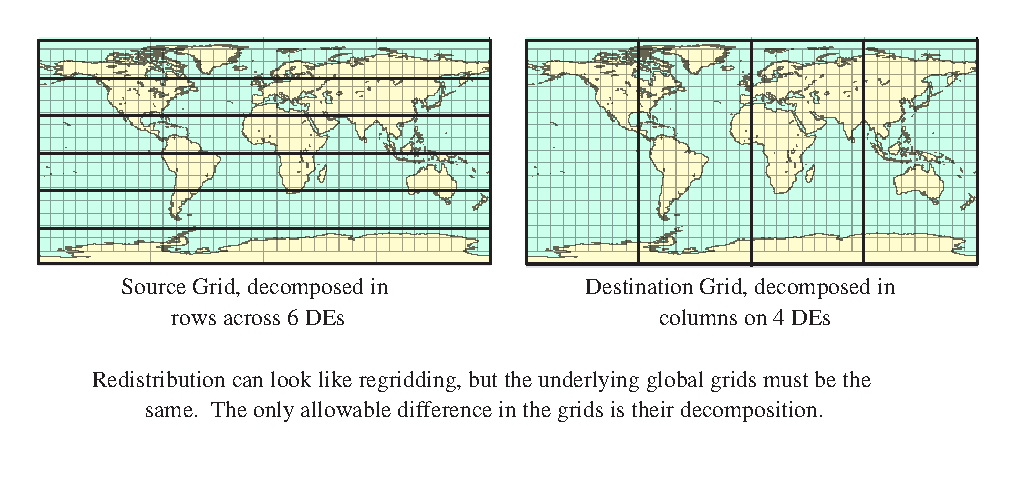
\includegraphics{Redist}}
\label{fig:Redist}
\caption{Illustration of redistribution of data. }
\end{figure}
\end{center}

Redistribution methods involve only data movement; no interpolation, data
binning, or averaging is performed.  For data associated with physical locations
on a IGrid, this means the source and destination IGrids must have identical
global coordinates.  Like Haloing and other high level communication routines,
Redistribution is supported at the Array, Field, and FieldBundle levels. 

